%%This is a very basic article template.
%%There is just one section and two subsections.
\documentclass{article}
\usepackage[a4paper, margin=2.5cm]{geometry}
\usepackage{amsmath}
\usepackage{amssymb}
\usepackage{caption}
\usepackage{placeins}
\usepackage{graphicx}
\usepackage{subcaption}
\usepackage{setspace}
\usepackage{float}
\usepackage{wrapfig}
\usepackage{pdfpages}
%\usepackage[active,tightpage]{preview}
\usepackage{natbib}
\bibpunct{(}{)}{,}{a}{}{;} 
\usepackage{url}
\usepackage{nth}
\usepackage{authblk}
\usepackage{blindtext}
% for the d in integrals
\newcommand{\dd}{\; \mathrm{d}}
\newcommand{\tc}{\quad\quad\text{,}}
\newcommand{\tp}{\quad\quad\text{.}}
\newcommand{\ra}{\rightarrow}
\def\lsub#1#2%
  {\mathop{}%
   \mathopen{\vphantom{#2}}_{#1}%
   \kern-\scriptspace%
   #2}
\def\lsup#1#2%
  {\mathop{}%
   \mathopen{\vphantom{#2}}^{#1}%
   \kern-\scriptspace%
   #2}

\defcitealias{HMD}{HMD}
\defcitealias{HFD}{HFD}
\newcommand\ackn[1]{%
  \begingroup
  \renewcommand\thefootnote{}\footnote{#1}%
  \addtocounter{footnote}{-1}%
  \endgroup
}
\newcommand\todo[1]{\textcolor{red}{[TODO: #1]}}
\newcommand\high[1]{\colorbox{yellow}{#1}}
\begin{document}

%\title{Macro patterns in the shape of aging}
\title{Boom, echo, pulse, flow\\ \small (Open version)}
\author[1]{Tim Riffe\thanks{riffe@demogr.mpg.de}}
\author[1]{Kieron Barclay}
\author[1]{Christina Bohk-Ewald}
\author[2]{Sebastian Kl\"uesener}
\affil[1]{Max Planck Institute for Demographic Research}
\affil[2]{Bundesinstitut f\"ur Bev\"olkerungsforschung}
\maketitle

\begin{abstract}
Human population renewal starts with births. Since births can happen at any
time in the year and over a wide range of ages, demographers typically imagine
the birth series as a continuous flow. Taking this construct literally, we
visualize the birth series as a flow. A long birth series allows us to
juxtapose the children born in a particular year with the children that
they in turn had over the course of their lives, yielding a crude notion of
cohort replacement. Macro patterns in generational growth define the meandering
path of the flow, while temporal booms and busts echo through the flow with the
regularity of a pulse.
\vspace{1em}

{\bf Keywords:} Fertility, Population structure, Population momentum, Population renewal, Data visualization
\end{abstract}

\onehalfspacing
\section{Introduction}
Usually demographers think of fertility as an age-regulated process. In any case it is
bounded by menarche and menopause, both of which are anchored to age. These anchors may
move, but not far or fast. And between these bounds, at least within acceptably homogeneous subpopulations, fertility patterns appear to conform to some regular schema. Since births can happen at any time throughout the year, and since demography usually deals in large numbers, it is common to imagine the birth flow as a continuous stream. This is so not only as a pragmatic assumption to allow for calculus, but it also gives us a heuristic understanding of fertility as a smoother of population structure \citep{arthur1982ergodic}. In this treatment, we retreat from rates, the material of projections, to the absolute number of babies born, the raw material of population renewal. 

We aim to represent a historical view of Sweden's historical birth series in a single multilayered visualization. The birth series is rendered as a flow, for the sake of beauty, and to invite newcomers and curious minds deeper into the discipline of demography. This image entails investment from the viewer, and this manuscript serves as a protracted legend and caption. Intellectual payoffs include a simultaneous sense of long term patterns of generational mixing and generational replacement, medium term baby booms and echos, and the short term shocks of population momentum. We challenge experienced demographers to relate this image to the Lexis diagram, to imagine how the picture would change if fertility were indexed to fathers' age, and to reimagine this image of aggregates as immense set of lineages.

We use birth count data from Sweden, covering a total of 241 occurrence years from 1775 to 2016. Data for the years 1891 to 2016 is taken directly from the \citet{HFD} without further adjustment. We augment the HFD series in both directions, including newly digitized data for the period 1775 to 1890 \citep{sgf1907}, which we have graduated and adjusted. We describe these adjustments in Appendix~\ref{sec:dataprep}. To complete our picture, we project the fertility of cohorts whose fertility careers are still incomplete (1972-2016) through age 45. We describe the details of this projection in Appendix~\ref{sec:proj}. The temporal spread from the earliest mother cohort in our final data set (1721) to the latest offspring cohort (2061) is 341 years.

\section{Age and cohort-structured birth count distributions}
A picture of the births in a year is for demographers most instinctively broken down by the age of mothers who gave birth in that year, Fig.~\ref{fig:agemother}, or by the year of birth of mothers Fig.~\ref{fig:cohmother}. These two distributions are essentially identical, but appear as mirror images if chronological time is enforced in $x$.

\begin{figure}[ht!]
\begin{subfigure}[t]{0.5\textwidth}
        \centering
        \includegraphics[width=\textwidth]{Figures/Fig11900MotherAge.pdf}
        \caption{Births in 1900 by age of mother}
        \label{fig:agemother}
\end{subfigure}
~
\begin{subfigure}[t]{0.5\textwidth}
        \centering
        \includegraphics[width=\textwidth]{Figures/Fig11900MotherCohort.pdf}
        \caption{Births in 1900 by year of birth of mother}
          \label{fig:cohmother}
\end{subfigure}
\caption{Births in a year structured by mothers' age versus mothers' year of birth are a
reflection over $y$ and shift over $x$. Count distributions such as this may be jagged, even if the underlying rate distributions are smooth, due to population structure. The deficit around age 31 in \ref{fig:agemother} is due to a smaller number of potential mothers: the 1871 birth cohort was smaller than the surrounding cohorts.}
\end{figure}

If one disposes of a long-enough time series of births classified by mothers' year of birth, then one may further examine and break down the full reproductive career of the cohort of individuals born in a particular year. Since the childbearing of a cohort is spread over a synchronous span of ages and years, the classification by age (Fig.~\ref{fig:age1900mother}) or year (Fig.~\ref{fig:year1900}) yields identical and redundant distributions.

\begin{figure}[ht!]
\begin{subfigure}[t]{0.5\textwidth}
        \centering
        \includegraphics[width=\textwidth]{Figures/Fig11900IDAge.pdf}
        \caption{Births from mothers born in 1900 by age of mother}
        \label{fig:age1900mother}
\end{subfigure}
~
\begin{subfigure}[t]{0.5\textwidth}
        \centering
        \includegraphics[width=\textwidth]{Figures/Fig11900IDYear.pdf}
        \caption{Births from mothers born in 1900 by year}
          \label{fig:year1900}
\end{subfigure}
\caption{Births of a cohort structured by mothers' age versus mothers' year of birth are a
shift over $x$. The births over the life of a cohort more often resemble the smoothness of fertility rate schedules,}
\end{figure}

The births in a year are classified by mothers' cohort, i.e. cohort \emph{origins} in Fig.~\ref{fig:cohmother}, whereas the births \emph{from} a cohort are classified \emph{to} time in Fig.~\ref{fig:year1900}. The two distributions are different in kind, but relatable and both on a common scale. A fuller representation of their relationship would place them as two disjoint distributions on the same timeline, as in Fig~\ref{fig:juxt}.

\begin{figure}[ht!]
 \centering
        \includegraphics[width=\textwidth]{Figures/Fig31900juxt.pdf}
        \caption{The cohort distribution of mothers who gave birth in 1900 and the births from mothers born in 1900 by year. These two distributions link three generations.}
          \label{fig:juxt}
\end{figure}

The two distributions in Fig.~\ref{fig:juxt} are related, and of comparable scale, but different in kind. The $x$ coordinate of the left distribution is indexed to mothers' birth cohort, whereas the $x$ coordinate of the right distribution is indexed to child cohort, occurrence year. In this way the $x$ coordinates belong to grandmothers and grandchildren, where the \emph{ego} generation is 1900. These are two quantities that we may wish to compare in various ways to get a better feel and understanding of the Swedish birth series. 

For the case of these Swedish data, we have 241 such distribution pairs, making single-axis rendering impractical. An honest attempt might look like Fig.~\ref{fig:reflect1}, where we reflect the Fig.~\ref{fig:juxt} left distribution over $y$ (\textbf{A}), keeping the Fig.~\ref{fig:juxt} right-side distribution on top (\textbf{B}). These two distributions are linked by the year 1900, which of course overlaps with neither of them. In this representation, \textbf{A} and \textbf{B} are re-drawn for each possible ego year (1775-2016), and therefore imply a large sequential set of overlapping distributions. Each \nth{20} distribution is highlighted, but despite attempts to make this graph legible, i) the high degree of overlapping and ii) the spatial dissociation of each \textbf{A} --- \textbf{B} pair makes the intended comparison difficult over the series.

\begin{figure}[ht!]
 \centering
        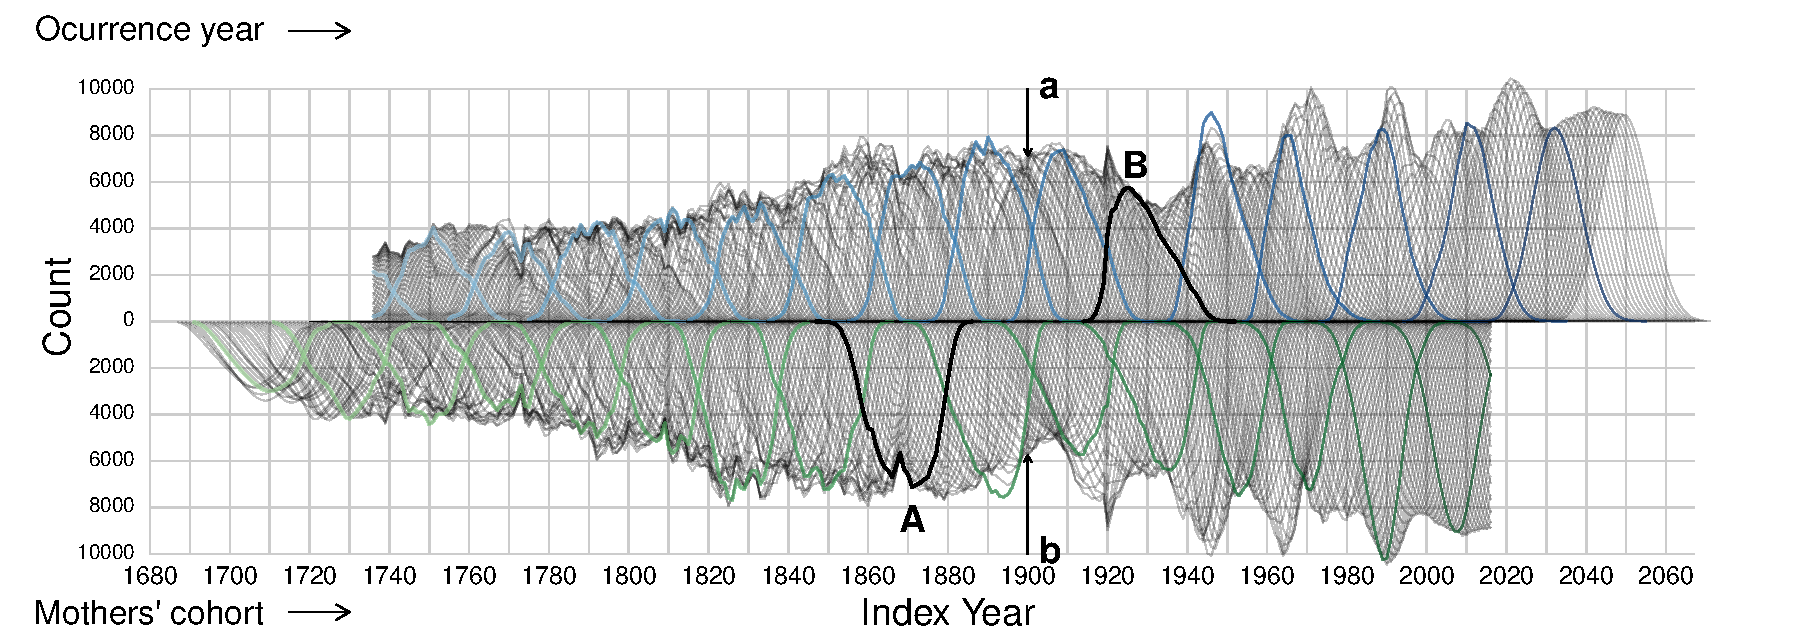
\includegraphics[width=\textwidth]{Figures/FxFlowReflect.pdf}
        \caption{Two time series of birth count distributions. The top series is composed of offspring distributions of mother cohorts over time, indexed to occurrence years. The bottom series is composed of the offspring of a year indexed to mothers' birth cohorts. \textbf{B} is the offspring of mothers from the 1900 cohort indexed in $x$ to occurrence year, and \textbf{A} are the births occurred in 1900 indexed in $x$ to mothers' birth cohorts. The cross-section \textbf{a} gives \textbf{A} and the cross-section \textbf{b} gives \textbf{B}.}
          \label{fig:reflect1}
\end{figure}

Fig.~\ref{fig:reflect1} produces at least two noteworthy artifacts that we may wish to preserve and clarify. 1) First order differences in the top series appear to cascade into the lower series--- This derives from a specific kind of population momentum \citep{keyfitz1971momentum}: larger cohorts have more offspring than smaller neighboring cohorts and vice versa, sudden fertility rate changes notwithstanding. 2) The composition of \textbf{A} in the bottom series is implied by the cross-section \textbf{a} of the top series, and the composition of \textbf{B} is implied by the cross-section \textbf{b}. This observation deserves further elaboration: The curve \textbf{A} is composed of all the births in 1900 indexed \emph{back} to mothers' cohorts. Each point on the curve \textbf{A} comes from a different top-axis distribution as it crosses the year 1900 (and vice versa for the bottom). The cross-section of curves \textbf{a} is therefore a redundant encoding of the single highlighted curve \textbf{A}. The cross-section \textbf{b} is a redundant encoding of \textbf{B} in the same way. While \textbf{A} and \textbf{B} are disjoint, and difficult to relate, \textbf{a} and \textbf{b} share a single $x$ coordinate, and so may lend themselves to comparison. The ``problem'' with the cross-sections \textbf{a} and \textbf{b} is that points from the corresponding distributions \textbf{A} and \textbf{B} are overlapped due to collapsation on a single $x$ coordinate. It is basically impossible to work out what \textbf{A} (\textbf{B}) might look like if presented only with \textbf{a} (\textbf{b}) and its surroundings. 
% Q: should the 'pointers' for a and b actually be drawn on top of the data series, as of a cross-section?
\pagebreak
% text above pushes whole thing down
\begin{wrapfigure}{r}{0.5\textwidth}
 \centering
        \includegraphics[width=3in]{Figures/FigReflection.pdf}
        \caption{The 1900 cohort as a composite bar with its offspring reflected over $y$. The size of each bar stacked in the top composition is proportionate to the area of its corresponding polygon in the left distribution of Fig.~\ref{fig:juxt}. The size of each bar stacked in the lower composition is proportionate to the area of its corresponding polygon in the right distribution of Fig.~\ref{fig:juxt}.}
          \label{fig:refl}
\end{wrapfigure}
% text under goes to the left then builds down
In this way the two distributions that we might wish to compare for a given ego
year are already available at a like coordinate, but comparison is stifled by
overplotting. If instead we stack the slices that are indecipherably overlapped
in \textbf{a} (and likewise for \textbf{b}) we get something like that shown in
Fig.~\ref{fig:refl}, cumulative birth distributions.\footnote{Young mothers are
on top and older mothers on bottom for both distributions. It would also make
sense to plot increasing (or decreasing) ages emanating out from the centerline
in both directions.} Here the total bar length is proportional to the total
cohort (offspring) size, and stacked bins reflect 5-year mother cohorts
(occurrence years). From this representation it is clear that mothers born in the
20 years between 1860 and 1880 produced the bulk of the 1900 cohort (86\%),
which itself produced the majority of its offspring in the 20 years between 1920
and 1940 (90\%). It is also quite visible that the 1900 cohort did not replace
itself in a crude sense: 138,139 babies formed a cohort whose mothers gave birth
to 95,379 babies over their lifecourse, a crude replacement of 69\%. Other
perspectives on reproduction that account for survival and attrition of the
mother cohort through migration would give a more optimistic assessment. The key
feature of Fig.~\ref{fig:refl} is that the two distributions that were disjoint in Fig.~\ref{fig:juxt} and hard to pick out in Fig.~\ref{fig:reflect1} can now be associated at a common $x$ coordinate. This virtue allows us to view the time series of Fig.~\ref{fig:reflect1} with greater clarity and perhaps reveal some macro properties of the history of Swedish natality.

Fig.~\ref{fig:foldout} is a depiction of the exercise of Fig.~\ref{fig:refl}, cohort bars on top reflected with offspring bars on the bottom. Equal bounded bins from Fig.~\ref{fig:refl} are joined into continuous regions. For the top region, filled polygons represent the births of mothers from quinquennial cohorts, spread over time. For the bottom region, filled polygons represent the mother-cohort origins of the births in quinquennial periods. The darkness and saturation of polygon fill colors are approximately proportional to the total births in the polygon (and therefore true to grayscale printing), whereas hue is irrelevant. In this way, darkness and saturation on the top are proportional to total height (with respect to baseline) on the bottom, and vice versa. 

The meandering baseline of Fig.~\ref{fig:foldout} is proportional to a smoothed time series of the crude cohort replacement rate. We overlay a horizontal line to indicate periods of approximate growth, replacement, and contraction. Periods where the meandering $x$-baseline is above this line (ca 1780 to 1860) indicate crude growth, and periods below the horizontal reference line (ca 1870 to 1930) indicate crude generation contraction. The nineteenth Century was characterized by steady replacement by this measure.

To aid the viewer with interpretation, we overlay a known lineage of five female generations,\footnote{This lineage can be located in the public domain on \url{https://www.geni.com/people/Karin-Ottolina-Landsten/6000000022470480183}.} where $x$ position is exact to the year, $y$ position in the top region is matched to the mothers cohort, and $y$ position in the bottom is matched to daughters' year of birth. Wider horizontal spacing between generations over time indicates increasing ages at maternity within this lineage (increasing from 23 to 39).



\begin{figure}
\centering
[fold-out figure 4$\times$a4 paper size at 100\% in separate pdf, about here.]
\includegraphics[scale=.3]{Figures/a4demonstration.png}
%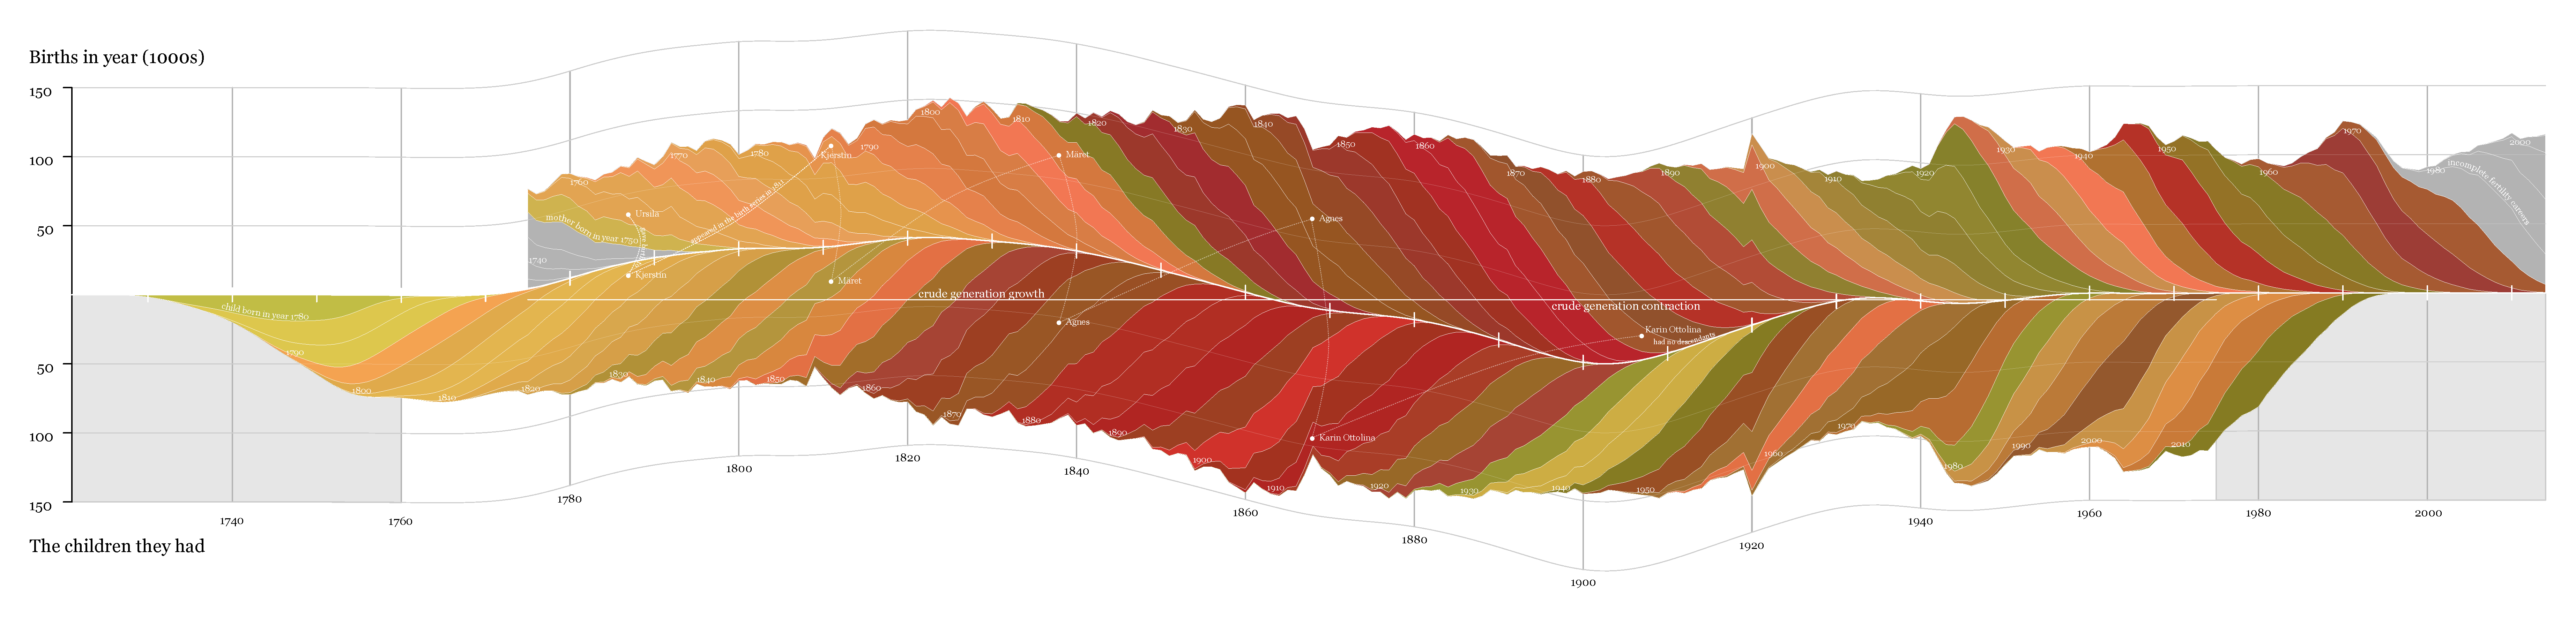
\includegraphics[scale=.9]{Figures/SwedenBirthFlowsManFoldout.pdf}
%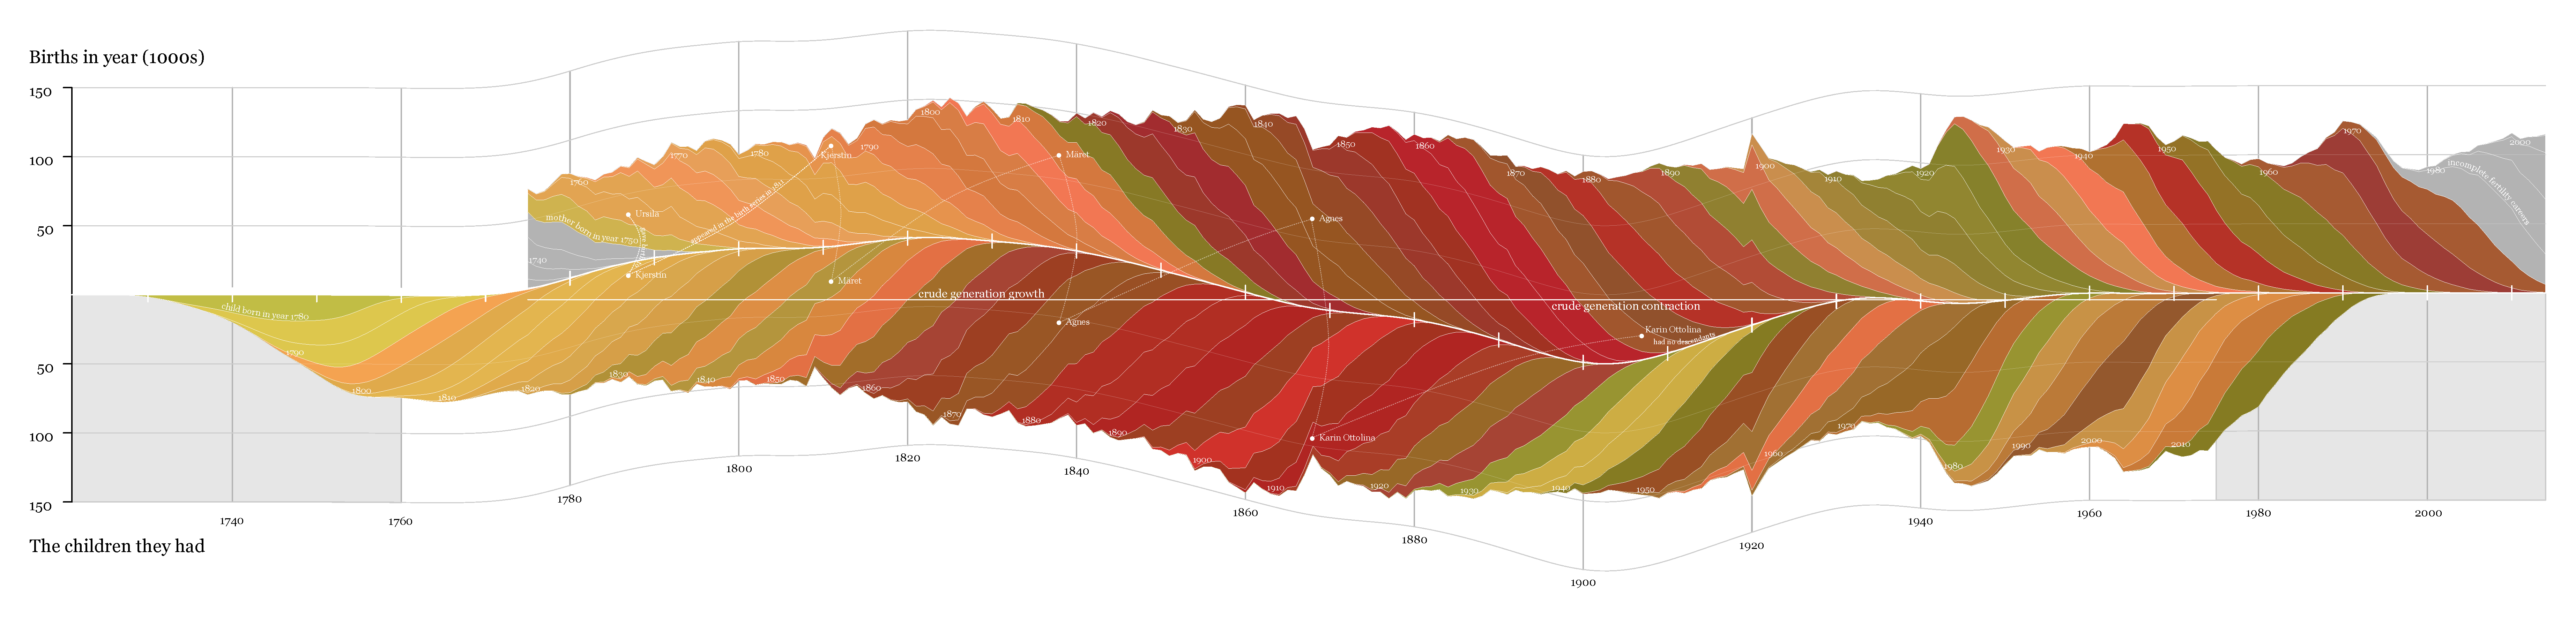
\includepdf[landscape]{Figures/SwedenBirthFlowsManFoldout.pdf}
\caption{A time series of the same graphical construct as presented in Fig.~\ref{fig:refl}. The $x$ axis now meanders proportional to a smoothed time series of the crude cohort replacement rate. Fill color darkness and saturation are approximately proportional to the total number of births in each birth distribution. The birth series now appears as a flow, but reveals echoes in cohort and offspring size, an odd periodicity in recent decades, and a long term dampening of the crude replacement rate. A 5-generation female lineage is annotated atop to serve as a guide.}
\label{fig:foldout}
\end{figure}

\subsection{Notes on visual form}
This visualization form derives from stacked area charts in general and river plots (theme river) and stream graphs in particular \citep{byron2008stacked}, but we wish to point out a few notable differences. Our birth flow visualization is composed of two separate stacked area graphs, where polygons appear in chronological order from left to right. If the top and bottom graph sections were vertically centered independently of one another, then these would comprise two ``river'' plots. Instead, the two series are squeezed together to share a $y$ coordinate at 0, and vertical centering is approximated on average by smooth baseline shifts. 

Different kinds of visual analytic tasks are probably penalized by this choice of form. For example, using the metrics proposed by \citet{thudt2016assessing}, we hypothesize that our visualization would perform poorly or moderately well in terms of ``individual discrimination'' because most birth distributions vary within the same order of magnitude. For example, it is not easy to visually discriminate the larger of ``number of children born in 1900 to mothers born between 1865 and 1869'' versus ``number of children that mothers born in 1900 had between the years 1925 and 1929'', (even though these share an $x$ coordinate) and such comparisons may be even more difficult the greater the distance in $y$ and $x$ between comparisons. 

If we wish to compare the area of polygons, our reflected axes are advantageous: for example, it is not easy to visually compare the area of the top-level polygon ``children to mothers born 1870-1874'' versus the area of the bottom-level polygon ``children born 1910-1914''. The darkness and saturation of polygon fill colors transmit this information, but the two fill colors are too similar to be very helpful in this case, especially since they are non-adjacent. However, these two polygons are redundantly encoded in a more comparable way: the first is coded to the average from 1870-1874 of the total height on the bottom $y$ axis, and the second is encoded the average total height from 1910-1914 on the top $y$ axis. This requires active decoding from the viewer, and such tasks are surely not quick, but likely result in precise judgments: The first polygon is larger than the second. For this kind of comparison, the polygons themselves are a distraction, as the same information is coded the height, but if there were no polygons then we would not be reminded that these two distributions are linked through time and through generations: the polygons overlap in $x$, and this is one of the prime data qualities that we wish to exemplify.

Again using the metrics of \citet{thudt2016assessing}, we presume to fare \emph{very} well in terms of ``stream comparison'', since the rendering of each birth distribution is matched to $x$, and also \emph{very} well in terms of aggregate discrimination of top versus bottom (because the meandering baseline gives this). Our visualization would presumably perform moderately well in terms of aggregate discrimination of top plus bottom, because river and stream plots also performed well on this metric, and our visualization resembles these in its manner of centering. In our case, the stream centering method brings the crude replacement ratio to the fore. On the other hand, certain visual tasks are augmented due to the nature of the data: visual discrimination of polygons is all but guaranteed. Chronological order is clear to the viewer. Even so, we accept high losses of value look-up ability, for the sake of an aesthetic welcome mat to those who wish to learn more about the fundamentals of demography in general and the Swedish birth flow in particular. Few small questions can be answered with this graphic, but some large ones may be inspired.

\section{Discussion}
\todo{To be continued...This section and the following analytic perspectives section are only temporary. We probably won't want to introduce new}
Several macro features come to the fore in this visualization. These are either known features of the Swedish birth series, or else merit further study. Echoes, booms, why is boom periodicity a recent phenomenon? Is there a dose-response to vertical reverberation in first derivative (can this be referred to as first or second order?) features.


\section{Analytic perspectives}
\todo{this sort of thing ought to inspire discussion, but the stuff presently in this section may not belong in the paper.}
A few macro patterns can be extracted from the data structure implied by the matrix $\mathbf{B}(c,t)$. 

\subsection{Analytic vignette 1}
An example of macro patterns that can be extracted from this data structure include two-distribution location distance statistics, as demonstrated in Fig.~\ref{fig:gmlag}. For each reference year in the range 1775 to \todo{1970} we have the mothers' cohort distribution and the next-generation childbirth year of occurrence distribution. Since both distributions are derived from the same table of counts by year of occurrence and mothers' age, it will help to use a simple notation, where the reference year is denoted with $r$, and following the index position convention $B(c,t)$ where mothers' cohort $c$ takes the first and year of occurrence $t$ the second position, respectively. In this way $B(c,r)$ are the births in year $r$ to mothers from cohort $c$ and $B(r,t)$ are the births in year $t$ to mothers from cohort $c$ (offspring). In this way, the weighted mean intergenerational lag $\overline{m2}$ is defined as
\begin{equation}
\overline{m2}(r) = \frac{\sum\sum (B(c,r)*B(r,t)) * (c - t)}{\sum\sum B(c,r)*B(r,t)} \quad \mathrm{,}
\end{equation}
and like-weighted distance quantiles may also be derived, as displayed in Fig.~\ref{fig:gmlag}.

\begin{figure}
% fig from CompareDist.R
\includegraphics[scale=.6]{Figures/GMLag.pdf}
\caption{Time lag from mothers' cohort to next generation offspring year of birth, the \emph{grandmaternal lag}, referenced to central (ego) cohorts. Decimals indicate birth distribution quantiles, where the red line indicates the median, and the blue dashed line the mean. The lag decreased broadly by all measures by ca 7-8 years in the 100 ego years from 1850 to 1950. The interquartile, 95\% and 99\% ranges also compressed by about 1 year in the same period.}
\label{fig:gmlag}
\end{figure}

From Fig.~\ref{fig:gmlag} we learn that the mean two-generation maternal lag decreased in the mean and all quantiles in the 100 years from 1850 to 1950 by around 7 to 8 years. The interquartile, 95\% and 99\% spreads all decreased by about 1 year over the same period, and by more than another year in the following 20 years.

\subsection{Analytic vignette 2}
One of the most immediately visible features of Fig.~\ref{fig:foldout} is the propagation of first differences in $B(t)$ to $B(c)$. The 1920 cohort is a particularly visible example: There were 23560 more births in 1920 than in 1919, an increase of 20.4\%, and mothers from the 1920 cohort also gave birth to 20.7\% more babies than the 1919 cohort. Fig.~\ref{fig:rBcrBt} displays the relationship in proportional first differences between matched birth cohort and offspring size. For the most part, the size of such structural echoes is maintained 1:1 in cohort offspring.


\begin{figure}
% fig from StructuralEchoes.R
\includegraphics[scale=.6]{Figures/rBcrBt.pdf}
\caption{A roughly 1:1 does-response relationship in relative size of structural echo.}
\label{fig:rBcrBt}
\end{figure}

\subsection{Analytic vignette 3}
\todo{KB suggests highlighting changes in the distribution of maternal age.} This is an interesting take: indeed the outer profiles would end up being the same, but the filled polygons would look different. If we did both at once then it'd make a plaid feel. Worth thought. Age could map to some other color property within polygons? Note: the younger-older gradient isn't reflected over $x$, as chronology is enforced. That is, earlier years of birth of offspring mean young (outside on bottom), but earlier years of birth of mother means old (outside on top). So earlier on the outside moves to later on the inside of the flow, but the younger-older gradient rather follows a down-up pattern within both the top and bottom. So adding age to the picture would require further care. But that's not to say there couldn't be an entirely separate plot of the same data indexed to age. Of the plaid remix of APC, with `younger-to-older' or `older-to-younger' from the baseline outward. 


\FloatBarrier

\singlespacing
\bibliographystyle{plainnat}
  \bibliography{references} 
  
\pagebreak
\begin{appendix}
\section{Data sources and adjustments}
\label{sec:dataprep}
Data presented here are from three separate series. The first
contains birth counts in the period-cohort Lexis shape,
\texttt{SWEbirthsVV.txt}, as produced by the \citet{HFD} according to the Methods
Protocol \citep{hfd2015methods}. This file contains births by calendar year and
mother birth cohort for the years 1891 until 2016, and we use it as-is. A
second file contains births for occurrence years 1775 until 1890. These data are
age-period classified, and given in a mixture of age classes, with a
predominance 5-year age classes (especially for ages 20-50), but also sometimes
single ages (especially for ages 15-19), and time-varying top and bottom open
ages. A third time series derives from a projection of cohort fertility for the cohorts born \todo{1970-2016} [Check years].

\subsection{Adjustments to historical data}
It is this second file, with data covering years 1890 and earlier, that we have
adjusted in four main steps. First, births of unknown maternal age were redistributed proportionally to the distribution of births of known maternal age. Second, counts were graduated to single ages using the graduation method proposed by \citet{rizzi2015efficient} and implemented in \texttt{R} in the package \texttt{pclm}\footnote{The \texttt{pclm} package has since been extensively modified, and it is now called \texttt{ungroup} \citep{pclmR}}. Third, counts were shifted into period-cohort Lexis bins assuming that half of the births in each single age $x$ bin go to the lower triangle of age $x+1$ and half to the upper triangle of the age-reached-during-the-year (PC) parallelogram at age $x$, as diagrammed in Fig.~\ref{fig:AP2PC}.

\begin{figure}[ht!]
\centering
\begin{subfigure}{.3\textwidth}
  \centering
  \includegraphics[scale=.6]{Figures/App_split1.pdf}
  \caption{AP square bins}
  \label{fig:app1}
\end{subfigure}%
\begin{subfigure}{.3\textwidth}
  \centering
  \includegraphics[scale=.6]{Figures/App_split2.pdf}
  \caption{Split evenly to triangles}
  \label{fig:app2}
\end{subfigure}
\begin{subfigure}{.3\textwidth}
  \centering
  \includegraphics[scale=.6]{Figures/App_split3.pdf}
  \caption{Regroup to PC bins}
  \label{fig:app3}
\end{subfigure}
\caption{The count regrouping procedure for years 1776 to 1890, step three of data adjustment. Data are graduated to single ages (Fig.~\ref{fig:app1}), then split in half (Fig.~\ref{fig:app2}) and regrouped to period cohort (PC) bins (Fig.~\ref{fig:app3}).}
\label{fig:AP2PC}
\end{figure}
At this stage data are binned and Lexis-conformable with HFD data for years 1891 and forward. With data processed as of step three, one could produce two time series represented in Fig.~\ref{fig:foldout}, with a subtle artifact visible in Fig.~\ref{fig:toosmooth}. In area \textbf{A} of this figure, birth counts in age bins have been graduated using the previously mentioned pclm method, which has the usually-desired artifact of smoothness. For the affected range of years, mother cohorts are identified via the identity $C = P - A - 1$ .\footnote{One subtracts 1 because data are in period-cohort bins.} Since age patterns of counts are smooth, these sum in Lexis diagonals to a smooth time series of cohort total offspring, as seen in the profile of area \textbf{B} of the same figure. Area \textbf{C} of this figure delimits years 1876 until 1971, where both cohort and matched offspring sizes are directly observed, and where fluctuations would appear to co-vary quite strongly. In the first instance for reasons of aesthetic continuity, and in the second instance for the sake of a more sensible count graduation, we have opted to adjust the counts in area \textbf{B} to carry the pattern of fluctuation observed over cohort size from 1775 to 1890.

\begin{figure}[ht!]
\centering
 \includegraphics[scale=.6]{Figures/App_preAdjustment.pdf}
\caption{In reference years $\ge$ 1891 both births by year and cohort offspring are directly observed in single year bins, which means that the structural echo between total birth cohort and offspring size is preserved for reference years $\ge$ 1876  (\textbf{C}). Total per annum births in years $\le$ 1890 (\textbf{A}) are presumed accurate, and so first differences of these are observed. Offspring from cohorts born in years $\le$ 1876 (\textbf{B}) were partially (1836--1876) or entirely ($<$ 1836) born in years $\le$ 1890, implying a smooth redistribution over single years of mother cohorts. We wish to adjust the births in \textbf{B} to recuperate the kind of structural echo in \textbf{C}.}
\label{fig:toosmooth}
\end{figure}

This adjustment works by extracting the fluctuation pattern from \textbf{A} and transferring it to \textbf{B}. We do this by first smoothing the annual time series of total cohort size $B(t)$ according to some smoothness parameter, $\lambda$.\footnote{For the present case we've used a loess smoother, using the \texttt{R} function \texttt{loess()} with smoothing parameter $\lambda =$ \texttt{span}. It would be straightforward to swap this smoothing method out with a different one.} The ratio of $B(t)$ to the smoothed birth series $B(t)^s$ defines the multiplicative adjustment factor, $adj(t) = B(t)/B(t)^s$. Total offspring size $B(c)$ is then adjusted as $B(c)' = adj(t)*B(c), \mathrm{~for~} c = t$. Counts in single ages are then rescaled to sum to the original totals in 5-year age groups, and counts for years $>$ 1890 are unaffected. The smoothing parameter is selected such that the linear relationship in fractional first differences $rd(B(t)) = \frac{B(t+1)-B(t)}{B(t)}$ between the annual birth series and adjusted offspring series $rd(B(c)')$ for years 1775-1890 matches that for the reference years 1877-1971 as closely as possible. Specifically, we select $\lambda$ so as to minimize the sum of the difference in the slope and residual standard deviation for the periods before and after 1891. Further clarifications about this adjustment, and code for diagnostic plots can be found in the annotated code repository. The end effect is to adjust the series to look like Fig.~\ref{fig:better}.

\begin{figure}[ht!]
\centering
 \includegraphics[scale=.6]{Figures/App_postAdjustment.pdf}
\caption{The adjusted birth series. Annual total births $B(t)$ on top axis and annual total offspring $B(c)$ on bottom axis, with adjusted offspring counts $B(c)'$ outlined.}
\label{fig:better}
\end{figure}
\end{appendix}

We adjusted in this way for the sake of a more nuanced time series of total offspring, but this approach may be used to good effect in graduating age-structured counts (births, deaths, populations) whenever time series are long enough to permit information on birth cohort size to propagate through the Lexis surface. These aspects are visible to some degree in the shaded polygons of Fig.~\ref{fig:foldout} in years $<$ 1891.

\subsection{Projected birth counts}
\label{sec:proj}
\todo{complete when exercise done}
Offspring counts by year of occurrence, $B(c,t)$ are only fully observed for years $\le$ 1971. To complete the reflection, we have opted to project birth counts for cohorts whose fertility careers are incomplete. This is done by combining a projection of cohort fertility rates using the method proposed by \citet{de1985time} with a standard projection of population denominators (mortality projection too? Could also just take the pop projection from Statistics Sweden.). Light documentation to follow here, as well as an update of Fig.~\ref{fig:better}.

\subsection{Meandering baseline}
\label{sec:baseline}
A peculiar feature of Fig.~\ref{fig:foldout} is the meandering baseline, which replaces the standard straight-line $x$-axis. The baseline is derived from the crude cohort replacement rate $\mathbb{R}(c)$, defined as $\mathbb{R}(c) = B(c=r) / B(t=r)$. This measure is not a replacement for the classic measure of net reproduction $R_0$, which differs in a few key ways: i) crude replacement is not sex-specific (our birth series is composed of boy and girl births combined), whereas $R_0$ is typically defined for females only. ii) while births arise from fertility rates over the life course, the number of potential mothers over the life course is not a mere function of mortality, but of migration as well, and the Swedish birth series will have been affected by heavy out-migration from 1850 until the Second World War (cite SCB), and some in-migration in more recent decades. Cohort $R_0$ is purged of population structure such as this (except to the extent that subgroups have differential vital rates), whereas $\mathbb{R}(c)$ is not, and for this reason we call it \emph{crude}.

The series of $\mathbb{R}(c)$ is rather smooth without further treatment, save for 11 periodic breaks between 1970 and 1840, a period of rupture between 1865 and 1880, and another set of at least four breaks since the great depression in the 1930s. Rather than preserve these ruptures, we opt to smooth them out and instead capture long term trends in $\mathbb{R}(c)$ in the baseline. Fig.~\ref{fig:meander}. Keeping the baseline meander smooth minimizes the visual penalty in assessing the variation in $B(c)$ or $B(t)$ separately, but it enhances our ability to see the long term pattern.

\begin{figure}[ht!]
\centering
 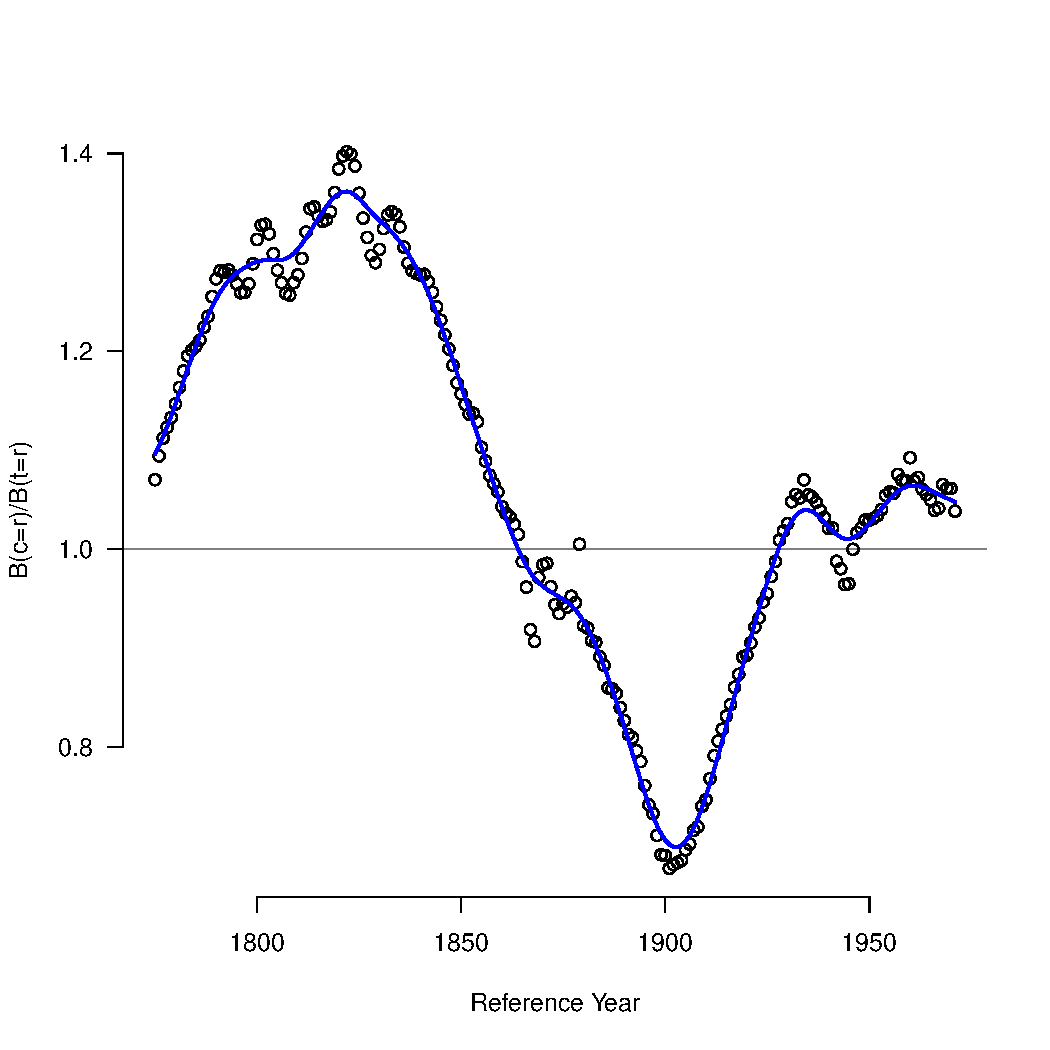
\includegraphics[scale=.6]{Figures/Meander.pdf}
\caption{The time series of crude cohort replacement, $\mathbb{R}(c)$, and its smooth pattern (blue line) on which the Fig.~\ref{fig:foldout} meandering baseline is based.}
\label{fig:meander}
\end{figure}


\end{document}
